\documentclass[tikz]{standalone}

\usetikzlibrary{automata}

\begin{document}
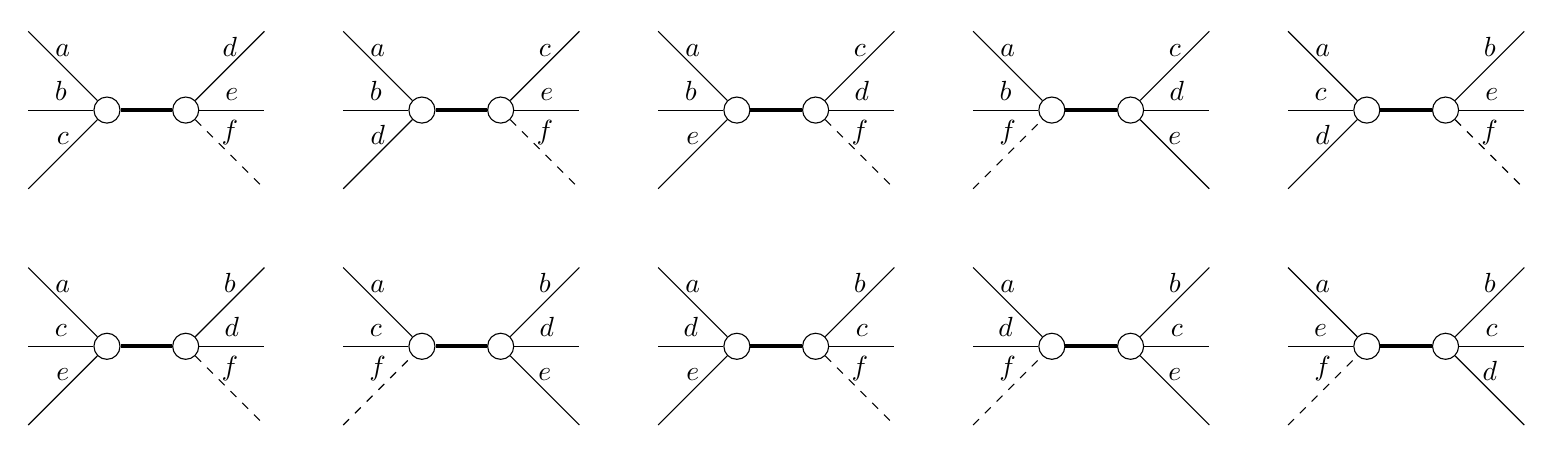
\begin{tikzpicture}
\tikzstyle{vertex}=[draw,shape=circle]
\path (0,0) node[vertex](x1){} (1,0) node[vertex](y1){};
\draw[line width=1.5pt] (x1) -- (y1);
\draw[] (-1,1) -- node[above] {$a$} (x1);
\draw[] (-1,0) -- node[above] {$b$} (x1);
\draw[] (-1,-1) -- node[above] {$c$} (x1);
\draw[] (y1) -- node[above] {$d$} (2,1);
\draw[] (y1) -- node[above] {$e$} (2,0);
\draw[dashed] (y1) -- node[above] {$f$} (2,-1);

\path (4,0) node[vertex](x1){} (5,0) node[vertex](y1){};
\draw[line width=1.5pt] (x1) -- (y1);
\draw[] (3,1) -- node[above] {$a$} (x1);
\draw[] (3,0) -- node[above] {$b$} (x1);
\draw[] (3,-1) -- node[above] {$d$} (x1);
\draw[] (y1) -- node[above] {$c$} (6,1);
\draw[] (y1) -- node[above] {$e$} (6,0);
\draw[dashed] (y1) -- node[above] {$f$} (6,-1);

\path (8,0) node[vertex](x1){} (9,0) node[vertex](y1){};
\draw[line width=1.5pt] (x1) -- (y1);
\draw[] (7,1) -- node[above] {$a$} (x1);
\draw[] (7,0) -- node[above] {$b$} (x1);
\draw[] (7,-1) -- node[above] {$e$} (x1);
\draw[] (y1) -- node[above] {$c$} (10,1);
\draw[] (y1) -- node[above] {$d$} (10,0);
\draw[dashed] (y1) -- node[above] {$f$} (10,-1);

\path (12,0) node[vertex](x1){} (13,0) node[vertex](y1){};
\draw[line width=1.5pt] (x1) -- (y1);
\draw[] (11,1) -- node[above] {$a$} (x1);
\draw[] (11,0) -- node[above] {$b$} (x1);
\draw[dashed] (11,-1) -- node[above] {$f$} (x1);
\draw[] (y1) -- node[above] {$c$} (14,1);
\draw[] (y1) -- node[above] {$d$} (14,0);
\draw[] (y1) -- node[above] {$e$} (14,-1);

\path (16,0) node[vertex](x1){} (17,0) node[vertex](y1){};
\draw[line width=1.5pt] (x1) -- (y1);
\draw[] (15,1) -- node[above] {$a$} (x1);
\draw[] (15,0) -- node[above] {$c$} (x1);
\draw[] (15,-1) -- node[above] {$d$} (x1);
\draw[] (y1) -- node[above] {$b$} (18,1);
\draw[] (y1) -- node[above] {$e$} (18,0);
\draw[dashed] (y1) -- node[above] {$f$} (18,-1);

\path (0,-3) node[vertex](x1){} (1,-3) node[vertex](y1){};
\draw[line width=1.5pt] (x1) -- (y1);
\draw[] (-1,-2) -- node[above] {$a$} (x1);
\draw[] (-1,-3) -- node[above] {$c$} (x1);
\draw[] (-1,-4) -- node[above] {$e$} (x1);
\draw[] (y1) -- node[above] {$b$} (2,-2);
\draw[] (y1) -- node[above] {$d$} (2,-3);
\draw[dashed] (y1) -- node[above] {$f$} (2,-4);

\path (4,-3) node[vertex](x1){} (5,-3) node[vertex](y1){};
\draw[line width=1.5pt] (x1) -- (y1);
\draw[] (3,-2) -- node[above] {$a$} (x1);
\draw[] (3,-3) -- node[above] {$c$} (x1);
\draw[dashed] (3,-4) -- node[above] {$f$} (x1);
\draw[] (y1) -- node[above] {$b$} (6,-2);
\draw[] (y1) -- node[above] {$d$} (6,-3);
\draw[] (y1) -- node[above] {$e$} (6,-4);

\path (8,-3) node[vertex](x1){} (9,-3) node[vertex](y1){};
\draw[line width=1.5pt] (x1) -- (y1);
\draw[] (7,-2) -- node[above] {$a$} (x1);
\draw[] (7,-3) -- node[above] {$d$} (x1);
\draw[] (7,-4) -- node[above] {$e$} (x1);
\draw[] (y1) -- node[above] {$b$} (10,-2);
\draw[] (y1) -- node[above] {$c$} (10,-3);
\draw[dashed] (y1) -- node[above] {$f$} (10,-4);

\path (12,-3) node[vertex](x1){} (13,-3) node[vertex](y1){};
\draw[line width=1.5pt] (x1) -- (y1);
\draw[] (11,-2) -- node[above] {$a$} (x1);
\draw[] (11,-3) -- node[above] {$d$} (x1);
\draw[dashed] (11,-4) -- node[above] {$f$} (x1);
\draw[] (y1) -- node[above] {$b$} (14,-2);
\draw[] (y1) -- node[above] {$c$} (14,-3);
\draw[] (y1) -- node[above] {$e$} (14,-4);

\path (16,-3) node[vertex](x1){} (17,-3) node[vertex](y1){};
\draw[line width=1.5pt] (x1) -- (y1);
\draw[] (15,-2) -- node[above] {$a$} (x1);
\draw[] (15,-3) -- node[above] {$e$} (x1);
\draw[dashed] (15,-4) -- node[above] {$f$} (x1);
\draw[] (y1) -- node[above] {$b$} (18,-2);
\draw[] (y1) -- node[above] {$c$} (18,-3);
\draw[] (y1) -- node[above] {$d$} (18,-4);
\end{tikzpicture}
\end{document}